\chapter{Etapa de búsqueda}
En esta etapa se realiza la búsqueda de instrucciones desde una memoria de solo lectura usando el  \ac{pc} y coloca esta en la etapa de ejecución por si hay algún salto. \cite{bib:Coad}
\section{Introducción}
 El \ac{pc} se incrementa de 1 y luego se reescribe el mismo el valor quedando listo para el próximo clock. Este valor es también guardado en la etapa de ejecución por si la instrucción a continuación es de salto, como por ejemplo \texttt{beq} (branch equal). (ver Figura \ref{fig:fetch})
 
\begin{figure}[H]
\centering
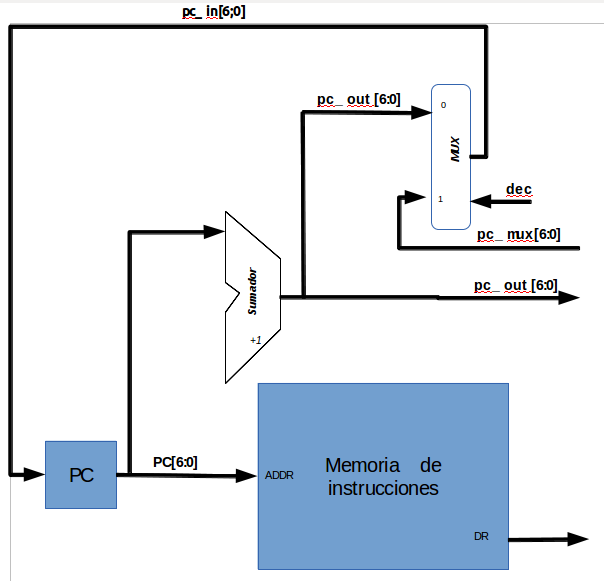
\includegraphics[scale=0.35]{Capitulo01/fetch}
\caption{Etapa de búsqueda}
\label{fig:fetch}
\end{figure}

Los cables que no están conectados son las entradas y salidas de acuerdo a la dirección de la flecha. En este caso \texttt{dec} y \texttt{pc\_mux} son las entradas al modulo. Las salidas son \texttt{pc\_out} y \texttt{DR}.

\begin{itemize}
	\item \texttt{dec}: Esta entrada es un multiplexor que elige entre los contadores de programa, que puede ser el que se viene incrementando de a uno en el módulo sumador \'o, si hubo un salto, el que se envió de la etapa de ejecución. 
	\item \texttt{pc\_mux}: Es el  \ac{pc} que viene modificado de la etapa de ejecución porque ocurrió un salto y ademas el decodificador se debe encargar de que el multiplexor lo elija.	
	\item \texttt{DR}: Son las instrucciones que entrega la memoria de acuerdo a la entrada que le brinda el \ac{pc}. 
	\item \texttt{pc\_out}: Esta es la salida del \ac{pc} que se traslada a la etapa de decodificación por si hay una instrucción de salto. 	
\end{itemize}

\section{Multiplexor}

El módulo multiplexor es binario, osea que solamente elige entre dos valores. En nuestro caso debe escoger entre el \ac{pc} que viene incrementado desde el modulo sumador o el que viene modificado por un salto desde la etapa de ejecución, ver código \ref{mux}. En la entrada del multiplexor entran 12 cables para que elija entre la parte alta y la parte baja, dependiendo de si es 1 o 0. Como lo programamos cuando \texttt{dec} esta en uno elige el \ac{pc}  que viene incrementado en el otro caso elige el que esta modificado por la etapa de ejecución.

\begin{figure}[H]
\centering
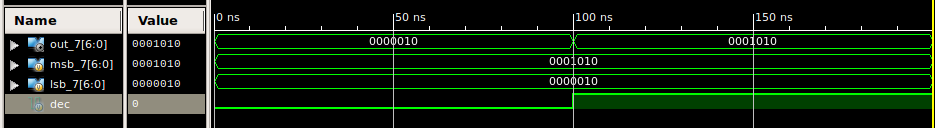
\includegraphics[scale=0.4]{Capitulo01/mux_test}
\caption{Testbench del multiplexor}
\label{fig:muxt}
\end{figure}

El codigo del testbench se puede ver en el apéndice \ref{mux_test} donde se modifica el valor de \texttt{dec} y en los cambios que ocurren se reflejan en la figura \ref{fig:muxt}, en un primer momento \texttt{dec=0} entonces la salida nos da \texttt{0000010} al cambiar el valor pasa a \texttt{0001010}.

\section{Incremento}
El modulo sumador simplemente incrementa el \ac{pc}, el código se muestra en el apéndice \ref{sum}  tiene solamente una entrada que es un bus de 7 bits y al valor que tiene es incrementado dentro del modulo. 

\begin{figure}[H]
\centering
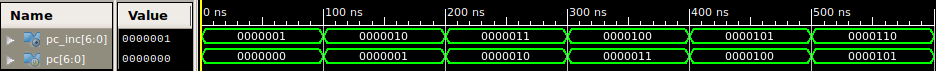
\includegraphics[scale=0.45]{Capitulo01/sum_test}
\caption{Testbench del sumador}
\label{fig:sumt}
\end{figure}

En el testbench contador de programa se va modificando de a uno, entonces la salida que en este caso es \texttt{pc\_inc} y esta ingresa en el registro del \ac{PC}. 

\section{Etapa de búsqueda con módulos integrados}
Finalmente generamos un modulo que integre los módulos anteriores generados y terminamos la etapa. El código de la etapa de búsqueda completo se puede ver en el apéndice \ref{fetch}. En este clock solamente el registro \ac{pc} cambiaría de valor. 

\begin{figure}[H]
\centering
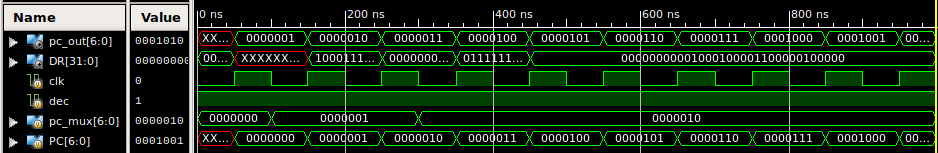
\includegraphics[scale=0.45]{Capitulo01/fetch_test}
\caption{Testbench del modulo fetch}
\label{fig:fetcht}
\end{figure}

Para entender que hace esta etapa podemos ver los cambios en la figura \ref{fig:fetcht}, debemos comenzar viendo que \texttt{PC} no tiene ningún valor y es el que le ingresara en el clock a la memoria de instrucciones, \texttt{pc\_out} tampoco contiene ningún valor y este entra en el multiplexor, la memoria de instrucciones se puede ver en \ref{a.coe}.  
En el primer clock ascendente como \texttt{dec} esta en uno, elije \texttt{pc\_mux} para escribir al \ac{pc} todos ceros o sea la primera direccion de memoria. El \ac{dr}  muestra  solo x porque en el clock anterior el \ac{pc} estaba en x y en la memoria no direcciona en ninguna posición valida. En el próximo clock ascendente ya el \ac{pc} contiene ceros por lo que automáticamente \texttt{pc\_out} va a tener el valor de \ac{PC} + 1, pero \texttt{dec} esta en 1 por lo que sigue eligiendo a \texttt{pc\_mux} que en el clock descendente anterior ya se le había aumentado el valor en 1 por lo que este valor va a ser ingresado en el próximo clock al \ac{pc} y \ac{dr} ya comienza a mostrar el primer valor de la memoria de instrucciones. Los siguientes clocks funcionan de la misma manera.

\lstinputlisting[label=a.coe, caption=Contenido de la memoria de instrucciones, captionpos=b]{Capitulo01/a.coe}